\documentclass[11pt]{article}

% PACKAGE USING
\usepackage[top = 1in, bottom = 1in, left = 0.75in, right = 0.75in]{geometry}
\usepackage{amsmath, amssymb, amsthm, amsfonts}
\usepackage{xcolor}
\usepackage{graphicx, subcaption}
\usepackage{url, hyperref}
\hypersetup{
    colorlinks = true,
    urlcolor = blue,
    citecolor = red
}
%\usepackage{biblatex}
%\addbibresource{references.bib}


\newcommand{\Q}{\mathbb{Q}}
\newcommand{\E}{\mathbb{E}}
\newcommand{\R}{\mathbb{R}}
\newcommand{\Acal}{\mathcal{A}}
\newcommand{\Fcal}{\mathcal{F}}
\newcommand{\transpose}{^{\intercal}}


\begin{document}

\begin{titlepage}
    \begin{center}
        \vspace*{5cm}
 
        \Huge{\textbf{Research Reading Assignment}}
 
        \vspace{0.5cm}
        \large{of the paper titled}\\
        \large{``Correlated Bandits for Dynamic Pricing via the ARC algorithm''}\\
        \large{by}\\
        \large{Samuel N. Cohen and Tanut Treetanthiploet}
             
        \vspace{1.5cm}
 
        \large{\textit{Prepared by,}}\\
        \large{\textbf{Subhrajyoty Roy}}\\
        \large{\textbf{MB1911}}
 
        \vspace{2cm}
             
        \textit{Assignment for Computational Finance course\\
        as a part of Master of Statistics curriculum}\\
        \vspace{0.5cm}
        \textbf{Session: } 2020-21\\
        Indian Statistical Institute, Kolkata

        \vfill
        
        \begin{flushright}
            \normalsize{\today}            
        \end{flushright}
    \end{center}
\end{titlepage}

\section{Introduction}

Multi-armed bandit problem~\cite{katehakis1987multi} depicts the situation of a gambler who enters into a casino with a finite amount of money and is posed with $k$ slot machines, each of which has a different probability of winning. The gambler is faced with the problem of allocating the resources efficiently to maximize his (her) expected payoff in the long run. The exploration-exploitation dilemma convolutes the problem: if the gambler finds a profitable slot machine and pours his all money into that, he is potentially losing the chances of gaining more from some other slot machines which he has not explored enough. This problem, originated from a theoretical probability background, has enormous real-life applications.

\begin{enumerate}
    \item A company has to understand which of the $k$ types of ads (or banners) to display to attract its customers and gain long term popularity. Here, the constant exploitation of a single banner might make it mundane for the customers.
    \item An exchange needs to allocate the underlying stock or assets among available $k$ types of financial instruments to make available for customers to purchase, to maximize its revenue.
    \item A person needs to allocate its resources (or money) to purchase $k$ different instruments on possibly different underlying, to maximize his gain. This is a typical portfolio optimization problem, which is dynamic in nature.
\end{enumerate}

\section{Mathematical Formulation of the Problem}

Multi-armed bandit problem starts with a space of actions $\Acal = \{ 1, 2, \dots K \}$. At time $t$, the gambler chooses action $A_t \in \Acal$, and if $A_t = k$, then he / she observes a random variable $Y_t^{(k)}$ and obtain a reward of $R^{(k)}(Y_t^{(k)})$, where the reward function may be different for different actions. There also exist a latent parameter $\Theta$ which specifies the distribution of all $\{ Y_t^{(k)} \}_{k=1, t=1}^{K, \infty}$ such that, $Y_t^{(1)}, \dots Y_t^{(K)}$ are conditionally independent given $\Theta$ for every $t$. An additional randomization over the action space $\Acal$ can be used to allow mixed strategies, by considering a sequence $(U_t)_{t=1}^{\infty}$ taking values in $\Delta^k = \{ (u_1, \dots u_K) : \sum_{i=1}^K u_i = 1 \text{ and } u_i \geq 0 \forall i \}$. Here, $i$-th component of $U_t$ denotes the probability of choosing action $i$ at round $t$.

There is a mutlitude of objective functions that one might choose to optimize with respect to the choice of $U_t$ such as

\begin{enumerate}
    \item Cumulative regret, $\mathcal{R}(\Theta, T, U_t) = \sum_{t=1}^{T} \left( \arg\max_k \E(R^{k}(Y_t^{(k)})) - \E_{U_t}(R^{(A_t)}(Y_t^{(A_t)})) \right)$.
    \item Discounted reward, $V(\Theta, \beta, U_t) = \sum_{t=1}^\infty \beta^{(t-1)}\E_{U_t}(R^{(A_t)}(Y_t^{(A_t)}))$.
\end{enumerate}

In the specific example of dynamic pricing considered by the authors~\cite{treetanthiploet2021correlated}, an exchange (or a store) has to determine which financial contracts to make available to maximize its revenue, let at the start of the day, the exchange needs to choose one of the contracts having features from the set $\{ x_1, x_2, \dots x_K \}$. On day $t$, with a chosen contract with feature $x_k$, $N_t^{(k)}$ customers visit the website of the exchange and $p(x_k)$ is the demand probability that each customer buys the contract. Assuming a GLM model for this probability yields

$$
Q_{i, t}^{(k)} \mid \Theta \sim_{IID} h(q)\exp\left( \phi(\Theta\transpose x_k )q - G(\phi(\Theta\transpose x_k)) \right), \dots i = 1, 2, \dots N_t^{(k)}
$$

\noindent which takes value $0$ or $1$ depending on whther $i$-th customer buys the contract or not. Assume, $h, \phi$ and $G$ are some known functions. Finally, a reward $R^{(k)}(\Theta, N_t^{(k)}, \sum_{i=1}^{N_t^{(k)}}Q_{i, t}^{(k)})$ is collected by the exchange which depends on both the number of persons visiting exchange website and the number of contracts sold.

\section{Solution to the Problem}

In each of the step $t$, there are two subproblems. In the first one, the store must make an inference of $\Theta$ given the history upto time $(t-1)$, i.e. $\Fcal_{t-1}$. In the second phase, based on this inference, the store must take an action $A_t$ which minimizes either the cumulative regret or maximizes the discounted reward.

\subsection{First Step: Inference about $\Theta$}

To solve the first step, assuming that the link function $\phi$ is differentiable, we define $\psi = (G' \circ \phi)^{-1}$ and note that by central limit theorem,

\begin{equation}
    \sqrt{n}\left( \dfrac{1}{n}\sum_{i=1}^n Q_{i,t}^{(k)} - \Theta\transpose x_k \right) \xrightarrow{d} \mathcal{N}\left( 0, 1/[G''(\phi(\Theta\transpose x_k))\phi'(\Theta\transpose x_k)^2] \right), \ n\rightarrow \infty
    \label{eqn:clt}
\end{equation}

\noindent Using eqn.~\eqref{eqn:clt}, one can show that $\Theta \mid \Fcal_{t-1} \sim \mathcal{N}(M_{t-1}, \Sigma_{t-1})$ where the posterior estimates of $M_{t}, \Sigma_t$ are updated by observing $N_t^{(k)}, Q_{i,t}^{(k)}$ as follows

\begin{align}
    M_t & = M_{t-1} + R_t^{(k)} (\Psi_t^{(k)} - M_{t-1}\transpose x_k)\Sigma_{t-1} x_k \label{eqn:update1}\\
    \Sigma_t & = \Sigma_{t-1} - R_t^{(k)} \Sigma_{t-1}x_k x_k\transpose \Sigma_{t-1} \label{eqn:update2}
\end{align}

\noindent where $\Psi_t^{(k)} = \dfrac{1}{n}\sum_{i=1}^n Q_{i,t}^{(k)}$ and $R_t^{(k)} = N_t^{(k)} V_t^{(k)} / (N_t^{(k)} V_t^{(k)} + x_k\transpose \Sigma_{t-1} x_k + 1)$, $V_t^{(k)} = [G''(\phi(\Theta\transpose x_k))\phi'(\Theta\transpose x_k)^2]$. The eqn.~\eqref{eqn:update1}-\eqref{eqn:update2} are simply Kalman filter type equations.

\subsection{Second Step: Taking optimized action}

There are numerous algorithms to maximize the reward in the long run, given the inference about the latent parameter has already been performed.

\begin{enumerate}
    \item Greedy algorithm to always take action $k = \arg\max \E_{\Theta \mid \Fcal_{t-1} \sim \mathcal{N}(M_{t-1}, \Sigma_{t-1})} R^{(k)}(\Theta, N_t^{(k)}, \sum_i Q_{i, t}^{(k)})$ may lead to suboptimal solution~\cite{russo2017tutorial}.
    \item $\epsilon$-greey algorithm~\cite{vermorel2005multi} takes the greey action with probability $(1-\epsilon)$, and chooses any other action at random with probability $\epsilon$. This ensures a balance between exploring results of new actions to ensure the inference about $\Theta$ is always updated.
    \item Explore-then-commit algorithm~\cite{rusmevichientong2010linearly} explores randomly for $[\epsilon T]$ rounds which is only used to update inference about $\Theta$, and then it keeps taking the greey action only.
    \item Thompson sampling~\cite{thompson1933likelihood} calculates the probability $\arg\max R^{(k)}(\Theta, N_t^{(k)}, \sum_{i=1}^{N_t^{(k)}}Q_{i, t}^{(k)}) = k$ for every choice of $k \in \Acal$. In other words, it calculates the probability under $\Theta \mid \Fcal_{t-1}$ that action $1$ is best, action $2$ is best and so on. Then, it samples an action $k$ according to that probability distribution. In other words, Thompson sampling reverses the maximization and expectation step in greedy algorithm.
\end{enumerate}

There are some other algorithms as well. The authors~\cite{treetanthiploet2021correlated} presents an improved \textbf{Asymptotic Randomized Control (ARC)} algorithm as another alternative to take this optimized action.  

\subsection{Asymptomatic Randomized Control Algorithm}

Asymptomatic Randomized Control (ARC) algorithm~\cite{cohen2020asymptotic} optimizes the choice of action $a$ to maximize the discounted reward (instead of minimizing cumulative regret). Denoting the term $f = [\E(R^{(k)}(Y_t^{(k)}) \mid \Fcal_{t-1})]_{k=1,2,\dots K}$ and $L^\lambda(a)$ as a special exploration term, the maximization of discounted reward leads to the solution of the fixed point equation as

$$
a = f(a) + \dfrac{\beta}{(1 - \beta)}L^\lambda(a), \ \text{ where } a \in \Delta^k = \{ (u_1, \dots u_K) : \sum_{i=1}^K u_i = 1, u_i \geq 0 \}
$$

\noindent where $f(a)$ is the expected reward over one time step if the action is chosen according to the distribution $\nu^\lambda(a) = (\nu^\lambda_1(a), \dots \nu^\lambda_K(a))$ over the action space $\Acal$, where $\nu_i^\lambda(a) = \exp(a_i/\lambda)/\sum_{j} \exp(a_j/\lambda)$. The choice of $L^\lambda(a)$ is used to motivate exploration rather than only committing towards the optimal action, in order to update inference about $\Theta$ over time. The expression of $L^\lambda(a)$ is given by,

\begin{figure}[h]
    \centering
    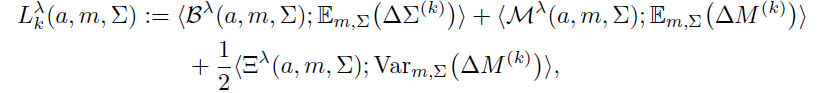
\includegraphics[width = 0.8\textwidth]{img1.PNG}
\end{figure}

\noindent where,

\begin{figure}[h]
    \centering
    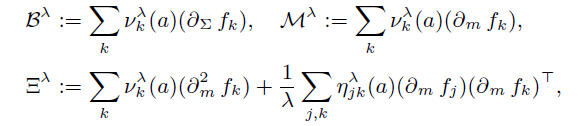
\includegraphics[width = 0.5\textwidth]{img2.PNG}
\end{figure}

\noindent with $\eta^\lambda_{jk}(a) = \nu^\lambda_j(a)(\mathbb{I}(j = k) - \nu^\lambda_k(a))$. The algorithm thus solves the fixed point equation to find $a$, and then obtains $\nu^\lambda(a)$ as the randomized action to choose in any timepoint $t$.

\section{Simulation Studies}

Dube and Misra~\cite{dube2017scalable}, in their experiment, randomly assigned one of ten different prices to $7867$ different customers who reached Ziprecruiter's paywall. Based on the data, the authors inferred the $\Theta$, and created $5000$ independent simulation of markets of one-year length, with $N_t \sim \text{Poisson}(270)$. Based on the simulations, they found that the ARC algorithm provides an optimal solution, while the existing methods do not reach the optimal solution even after sufficient trials. Also, ARC and Knowledge Gradient (KG) method achieves the optimal reward with a minimum number of changes in prices and hence is preferable over other algorithms.

\section{Conclusion and Comments}

\begin{enumerate}
    \item The authors avoid expressing enough motivation behind the ARC algorithm. However, if the bandits are correlated, and one of the bandits, even being costly, provides extremely crucial information about $\Theta$, ARC algorithm motivates to explore that.
    \item There is no clear indication of how the learning function came to be. Intuitively, it uses $\partial_\Sigma f_k$ which denotes the tradeoff between information gain about $\Theta$ and the loss of expected reward.
    \item The consideration that the probability of buying $p(c_k)$ is the same for every customer is a problem since it depends on particular user preferences.
    \item Also, $p(c_k)$ should depend on time $t$ as well, since there is usually a trend effect that motivates investors to buy a particular type of contracts (or on a particular asset) more.
    \item More simulations with different incoming distributions other than Poisson should be executed to understand whether the results are consistent. Since the theoretical guarantees only hold asymptotically, a large value of $N_t^{(k)}$ is required to make a reasonable inference.
    \item Usually, if $c_k$ is very high, the demand may be extremely low, and in some cases, all $Q_{i,t}^{(k)} = 0$. In such cases, a geometric model could prove useful.
\end{enumerate}

However, the approach presented by the algorithm is novel in the sense that it considers the problem where bandits are correlated with each other, which is of extreme practical importance since, in the dynamic pricing setup described in the paper, common information about a reasonable price range of the product is available to all customers.


\bibliographystyle{plain}
\bibliography{references.bib}

\end{document}